\section{Background}
\label{sec:background}
Despite recent interest, concerns about system power have existed since the dawn of computing. Some of the earliest valve-based computers had power draws comparable to modern supercomputers. The ENIAC machine dissipated 174 kW \cite{birnbaum:2000aa}, a figure which would not look out of place in the current Top 500 list, despite the fact this machine dates from 1947.\golden

When bipolar semiconductor technologies superseded thermionic valves in the 1950s and 60s the result was a dramatic reduction in system power consumption. Over time, manufacturing improvements delivered ever smaller transistors, yielding rapid increases in both performance and power density. Ultimately this resulted in chips which strained the limits of cooling technologies~\cite{jouppi:1994aa}. \golden

The use of bipolar semiconductors peaked in the early 1990s when they were replaced in turn with the Complementary Metal Oxide Semiconductor (CMOS) technology we still rely on today. CMOS was a mature technology which offered far superior energy consumption characteristics. It had been  overlooked previously as it was thought to be too slow for use in high-performance microprocessors. \golden

\begin{figure}[ht]
\centering
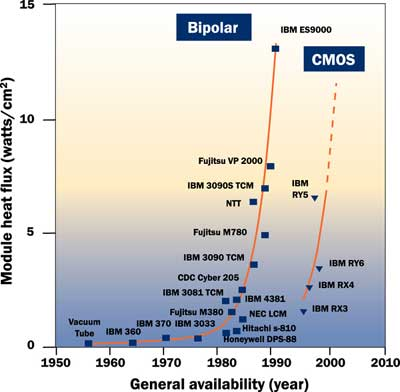
\includegraphics[width=0.9\linewidth]{Images/bipolarcmos.jpg}
\caption{Trends in module level power density, reproduced from \cite{chu:1999aa}. Copyright 1999 IEEE.}
\end{figure}
This pattern of improving hardware until physical limits forces a switch to new technologies is a recurring one. The previous iteration saw the widespread adoption of multi-core architectures, and once again we find ourselves coming up against fundamental limitations \cite{esmaeilzadeh:2011aa}. Unfortunately this time we lack a mature semiconductor technology or transformational architectural paradigm waiting in the wings. Researchers are therefore searching for alternative ways to combat the rise of power consumption whilst we await the emergence of the next fundamental shift in processor technology. \golden

System architects are already focussing on power efficient chip design, with recent innovations in areas including on-die voltage regulation \cite{burton:2014aa}, Dynamic Voltage and Frequency Scaling (DVFS) scheduling \cite{kwon:2013aa} and energy efficient heterogeneous cores~\cite{gupta:2012aa}.\golden

Performance engineers working with standard hardware are also beginning take note of this issue as it becomes increasingly central to scientific computing. It is their efforts to improve software power consumption that we hope to guide in this paper, and so we now limit our discussion to considering commodity CMOS chips with conventional architectures. \golden

The power draw of CMOS chips can be split into distinct components, the most significant of which are dynamic power and leakage power. Dynamic power is essentially the power consumed as logic gates change state while a processor performs work. Leakage power dissipation stems from the fact that at very small scales the insulating properties of silicon break down, allowing some current to flow even when gates remain inactive. Other forms of power dissipation exist, however their effects are relatively minor. \golden

\begin{equation}
\label{eq:totpwr}
P_{tot} = P_{dyn} + P_{leak} + P_{other}
\end{equation}
\begin{equation} 
\label{eq:dynpwr}
P_{dyn} \propto CV^{2}Af
\end{equation}
\begin{equation}
\label{eq:leakpwr}
P_{leak} \propto V\left(ke^{\frac{-qV_{th}}{ak_{a}T}}\right)
\end{equation}

Equations~\ref{eq:dynpwr} and \ref{eq:leakpwr} above give relations for dynamic and sub-threshold leakage power respectively. In Equation~\ref{eq:dynpwr}, C denotes load capacitance (a property influenced by wire lengths of on-chip structures), $V$ the supply voltage, $A$ the activity factor and $f$ the clock frequency. There is also a link between $V$ and $f$, as higher clock frequencies require higher supply voltages to sustain them. \golden

Equation~\ref{eq:leakpwr} is a simplified equation for sub-threshold leakage power. The new terms introduced in this equation include $T$, temperature, $V_{th}$, the transistor threshold voltage and $k$ the Boltzmann constant. The remaining parameters $q$, $a$ and $k_{a}$ capture CMOS logic design and fabrication characteristics. There several other sources of leakage energy, however we omit them here for brevity.\golden

Historically, dynamic power has been the biggest contributor to $P_{tot}$. Since the breakdown of Dennard scaling however leakage power has been on track to overtake it.  Sub-threshold and gate-oxide leakage dominate total leakage current, with both increasing exponentially as transistors shrink. Process improvements like the introduction of high-k dielectric materials~\cite{jan:2009aa} have kept leakage power in check over the last decade, however there is no avoiding the fact that insulating properties degrade as transistors shrink, allowing more current to leak. \golden

An important feature of the equations governing power draw is that only $P_{dyn}$ is influenced by software, in particular because it includes the $A$ term. Software can also indirectly effect both dynamic and leakage current if it triggers changes to clock frequency and therefore supply voltage. This effect is however primarily one of clock frequency rather than software and should be considered as such.\golden

The final thing to consider before we proceed to software optimization is the metric which is to be optimized. Code optimisation is a complex task during which developers rely on the support of a range tools and techniques. Up until now the overarching goal of performance engineers has been to minimize a single metric - run time. New metrics must be incorporated into these tools in order to support multi-objective optimization encompassing both power and runtime. \golden

Energy to completion is an obvious choice for domains where energy is severely restricted, for example in mobile platforms. That said, the fact that this metric fails to consider runtime limits its utility in scientific computing domains.\golden

The metrics often selected in practice are variants of the energy-delay product (EDP) \cite{gonzales:1995aa}. If either the runtime or energy consumption of a code increase then its EDP will increase proportionately as both components equally weighted. EDP can be defined in various equivalent ways:\golden

\begin{equation}
EDP = Energy \times Runtime
\end{equation}
\begin{equation}
EDP = Power \times Runtime^{2}
\end{equation}
\begin{equation}
EDP = Power \times (Instructions / MIPS)^{2}
\end{equation}

One criticism of EDP is the equal importance it assigns to power and runtime. Variants of EDP have been proposed which assign greater weight to the runtime component. The most frequently encountered of these are  energy-delay-squared product ($ED^{2}P$) and energy-delay-cubed product ($ED^{3}P$). \golden


 It can be argued that $ED^{2}P$ is a good choice when considering a fixed micro-architecture \cite{brooks:2000aa}. Briefly, equations \ref{eq:totpwr} and \ref{eq:dynpwr} show that $P_{tot} \propto CV^{2}Af + P_{leak} $, which can be approximated by $P_{tot} \propto V^{3}$ for a fixed system and workload. We also know that performance, clock frequency and voltage are all roughly proportional. As a result we have $Runtime^{3} \propto P_{tot}$. This demonstrates that $Power \times Runtime^{3}$, known as $ED^{2}P$, is a fair way to compare energy and performance efficiencies as the contributions of both factors are well balanced. \golden